\chapter{Background}
\section{Diffusion models}
%There are several components that are used to create an image with AI. The most impactful one of these is the prompt: this is a piece of text that describes what the image should look like. Then there are other parameters added on top of that. The guidance scale (CFG) configures how strictly the model is pulled towards the prompt. \\
%For the scope of this thesis, only FLUX.1 [dev] will be used. This is a subjective choice, based on the quality on the model and how easy it is to train LoRA's for FLUX.1 [dev]. FLUX.1 [dev] is a guidance-distilled model, however FLUX.1 [schnell] is a timestep-distilled model, trained to generate good results in 1-4 interference steps.
\subsection{Definition}
Diffusion models are a type of generative artificial intelligence model which is as of 2024 most used for computer vision tasks, such as image generation, inpainting, image denoising and video generation. These models are trained on a large dataset of images and captions, learning to gradually denoise an image from pure noise to a high-resolution image.

\subsubsection{Training and inner workings of diffusion models}
The training and deploying of a diffusion model can be broken down into 3 stages: the forward diffusion process, the reverse diffusion process and finally image generation.\\ During the forward diffusion process, an image from the data set is transformed into pure noise. The most common method is by iteratively injecting Gaussian noise until the entire data distribution is gaussian \autocite{noauthor_what_2024}.\\ The reverse diffusion process is where the actual machine learning takes place: the model learns to perform the reverse of the noising steps of the forward process and thus learns to denoise pure gaussian noise into an image.
\begin{figure}[H]
    \centering
    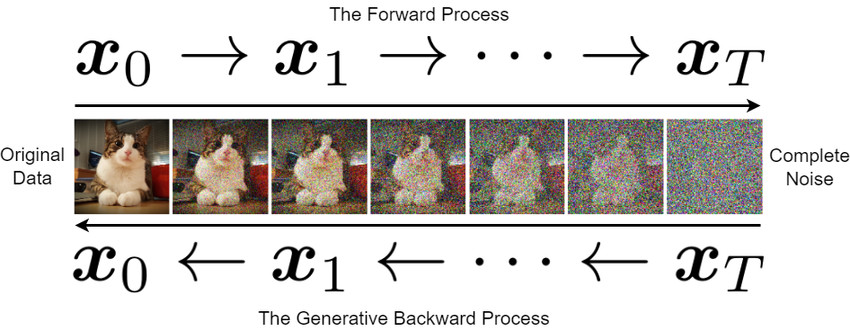
\includegraphics[width=0.8\linewidth]{Images/Background/The-forward-and-backward-processes-of-the-diffusion-model-The-credit-of-the-used-images.jpg}
    \caption{A visualisation of the forward and reverse diffusion process.}
    \label{fig:enter-label}
\end{figure}
Once the diffusion model has learned to estimate the amount of noise to be subtracted at each step, it can be used to generate new images. Inserting a slight element of randomness into this sampling process allows diffusion models to generate new images, that are not necessarily the same as the training images.
\subsubsection{Guided diffusion models}
A standard diffusion model can create high-quality variations of training images at random. Most practical uses of a diffusion model, however, require some control over the model's output. Guided diffusion models solve this problem by letting the user condition the generated images with a specific guidance.\\
The most common type of guided diffusion model is a text-to-image diffusion model, which lets users guide the generated images with a text prompt.\\
Methods for guided diffusion can be divided into two categories: Classifier-guided diffusion and classifier-free guidance. Classifier-free guidance has the benefit of enabling guidance for unseen image categories, whereas classifier-guided diffusion causes the diffusion model to only be able to condition outputs on the specific categories learned by the classifier.\\
Classifier-free guidance typically entails a two-stage model: in the first stage an embedding algorithm, like CLIP, creates an embedding for the prompt. In the second stage, a diffusion model uses this embedding to condition its output.
\subsubsection{Latent Diffusion models}
Conventional diffusion models are very good at generating images. However, they're slow and computationally expensive. These disadvantages were greatly reduced by latent diffusion models (\cite{rombach_high-resolution_2022}), starting with Stable Diffusion. \\
Rather than applying the diffusion process in pixel-space (i.e. directly to input images), these models first project the input to lower-dimensional latent space and apply the diffusion process there. The conversion of data from pixel space to latent space is done using a variational auto-encoder (VAE). The latent representation is then used as the input to the diffusion model. The output of the diffusion model, which is in the latent space, is finally upsampled to the desired image size using a decoder.
\subsection{Diffusion-based image generation models}
Over the last couple of years, Diffusion-based image generation models have become more and more popular, starting with the release of DALL-E by openAI in 2021. \\
\\
Generative image AI models come in two big categories: open-source and closed-source. Open-source models (e.g. stable diffusion and FLUX) can be downloaded through an online platform such as huggingface and used locally . Provided that one has access to a computer powerful enough to use these models, one can generate as many images as they like with these models. Closed-source models (e.g. Midjourney, Ideogram) ask a certain fee per month or per image generated, and can only be used through certain websites (e.g. fal.ai, replicate.com, midjourney.com, ideogram.ai).\\ 
\\

\subsubsection{Low-Rank Adaptation}
Low-rank adaptation, or LoRA in short, is a method to fine-tune models. Unlike full fine-tuning, this method uses less storage space; around a few hundred megabytes instead of many gigabytes. Training a LoRA takes on average only a few hours, depending on which hardware you use. These two properties make it an interesting tool to use for architects.

\subsubsection{ControlNet}
In the paper "Adding conditional control to text-to-image diffusion models", lvmin Zhang and coworkers from Stanford university introduced ControlNet, a 'neural network architecture to add spatial conditioning controls to large, pretrained text-to-image diffusion models' \cite{zhang_adding_2023}. ControlNet can be used to take the geometry from real images (such as sketches) and make the AI-generated images follow the same geometry. There are several 'preprocessors' which can freeze the geometry: in this paper, canny edge detection is used.
\subsection{Finetuning of diffusion models}
\subsection{Controlnet}